\documentclass[convert = false, tikz]{standalone}
\usepackage[utf8]{inputenc}
\usepackage{tikz}
\usetikzlibrary{automata, positioning, arrows}
 
\usepackage{../../../../style_automata}

% arara: pdflatex
% arara: latexmk: { clean: partial }
\begin{document}
    \tikzset{
    node distance=2cm and 2.5cm, % specifies the minimum distance between two nodes.
    initial text=start % sets the text that appears on the start arrow
    }
    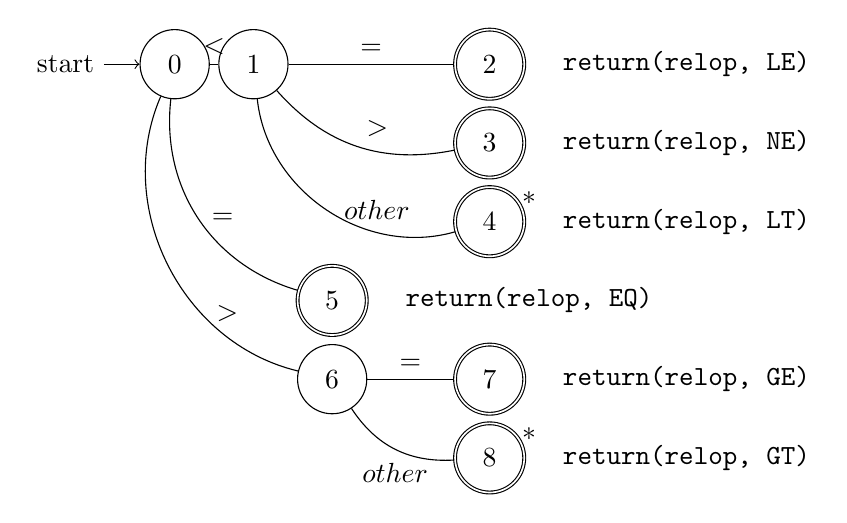
\begin{tikzpicture}
        \node[state, initial] (t0) {$0$};
        \node[state, right of=t0] (t1) {$1$};
        \node[state, accepting] (t2) at (4, 0) {$2$};
        \node (text2) at (6.5, 0) {\texttt{return(relop, LE)}};
        \node[state, accepting] (t3) at (4, -1) {$3$};
        \node (text3) at (6.5, -1) {\texttt{return(relop, NE)}};
        \node[state, accepting] (t4) at (4, -2) {$4$};
        \node (text4) at (6.5, -2) {\texttt{return(relop, LT)}};
        \node (star4) at (4.5, -1.7) {$*$};
        \node[state, accepting] (t5) at (2, -3) {$5$};
        \node (text5) at (4.5, -3) {\texttt{return(relop, EQ)}};
        \node[state] (t6) at (2, -4) {$6$};
        \node[state, accepting] (t7) at (4, -4) {$7$};
        \node (text7) at (6.5, -4) {\texttt{return(relop, GE)}};
        \node[state, accepting] (t8) at (4, -5) {$8$};
        \node (text8) at (6.5, -5) {\texttt{return(relop, GT)}};
        \node (star8) at (4.5, -4.7) {$*$};
        \draw (t0) edge[above] node{$<$} (t1)
        (t1) edge[above] node{$=$} (t2)
        (t1) edge[above, bend right=30] node[above right]{$>$} (t3)
        (t1) edge[above, bend right=50] node[right=0.1cm]{$other$} (t4)
        (t0) edge[above, bend right=40] node[right=0.05cm]{$=$} (t5)
        (t0) edge[above, bend right=50] node[below right=0.4cm and 0.5cm]{$>$} (t6)
        (t6) edge[above] node{$=$} (t7)
        (t6) edge[above, bend right=30] node[below=0.05cm]{$other$} (t8)
        ;
    \end{tikzpicture}
\end{document}